% Generated by tex/build_swebok_structure.py from tex/chapters/ch01/03_ソフトウェア要求の基礎.tex
\subsubsection{システム要求とソフトウェア要求}

\term{システム要求}は、ソフトウェアだけでなく、ハードウェア、ファームウェア、人、情報、手順、設備、サービス、支援要素を含むシステム全体に対する要求である。自動運転車、医療機器、工場制御、航空機システムのように、複数の要素が組み合わさる場合には、システム要求とソフトウェア要求を分けて扱うことが重要である。

\term{ソフトウェア要求}は、その大きなシステムの中で、ソフトウェア要素が満たすべき要求である。たとえば「車両は障害物を検知して安全に停止する」はシステム要求であり、その一部として「認識ソフトウェアは前方物体を一定時間内に分類する」といったソフトウェア要求が割り当てられる。

\begin{figure}[htbp]
\centering
\IfFileExists{assets/generated_figures/ch01/fig-ch01-04.png}{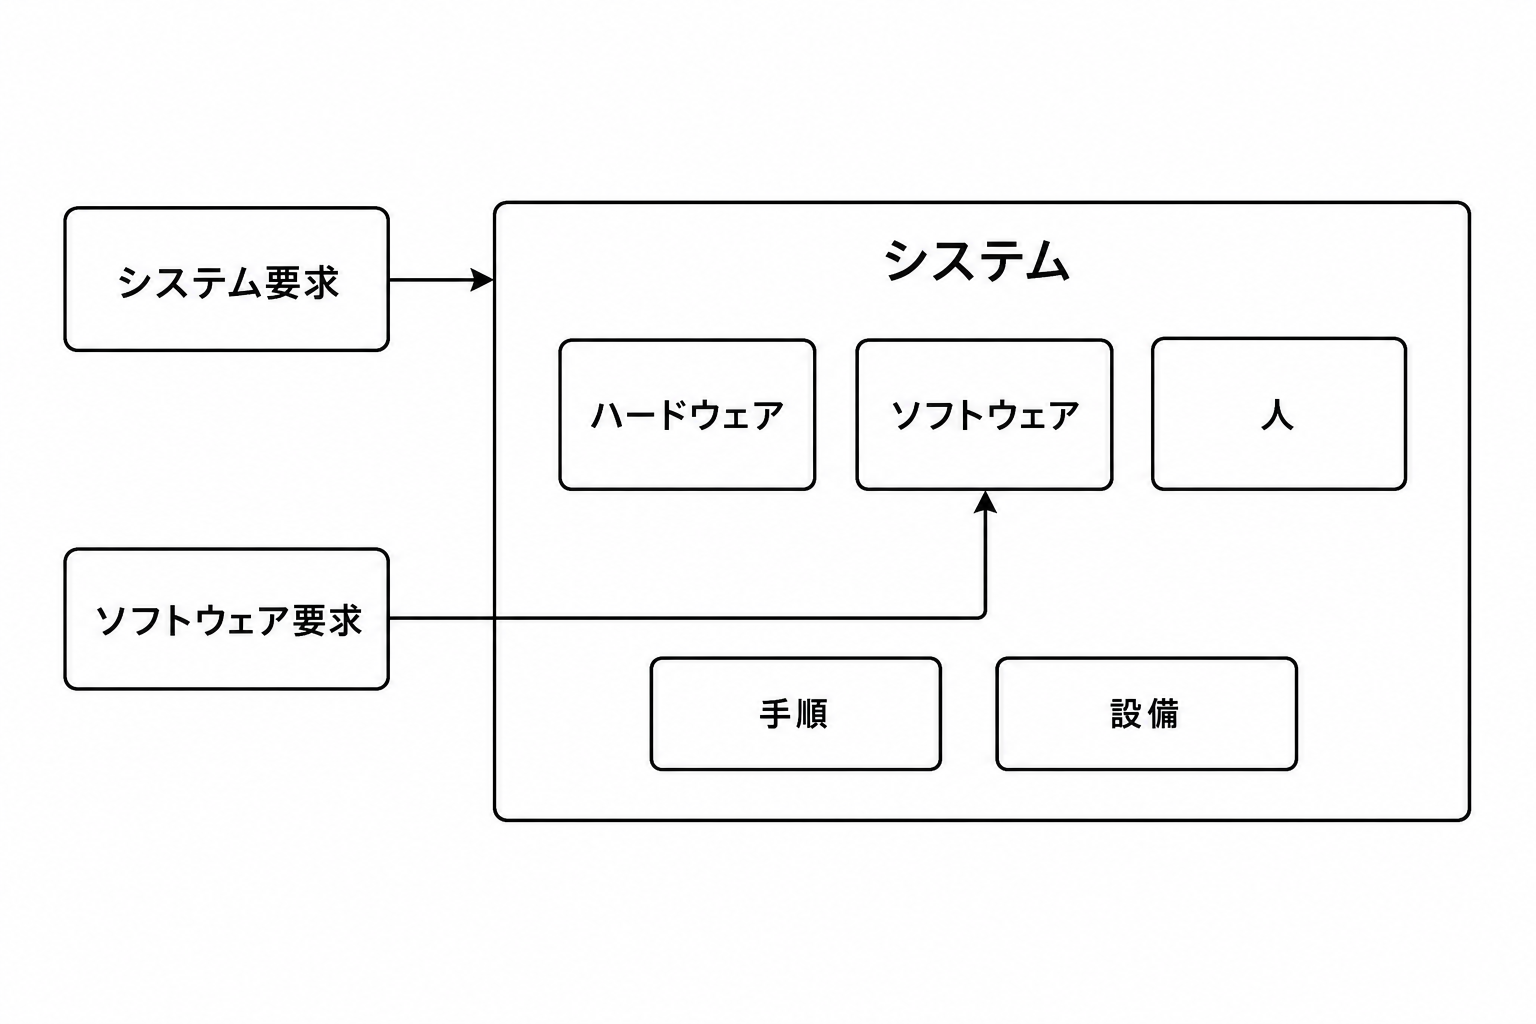
\includegraphics[width=0.96\linewidth]{assets/generated_figures/ch01/fig-ch01-04.png}}{\fbox{\parbox[c][48mm][c]{0.9\linewidth}{\centering 画像生成待ち\\システム要求からソフトウェア要求への割当図}}}
\caption{システム要求からソフトウェア要求への割当図}
\label{fig:ch01-04}
\end{figure}
